\documentclass[12pt]{amsart}

% %%%%%%%%%%%%%%%%%%%%%%%%%%%%%%%%%%%%%%%%%%%%%%%%%%%%%%%%%%%
% FONT ENCODING

\usepackage[T1]{fontenc}
\usepackage[utf8]{inputenc}
\usepackage{lmodern}

% %%%%%%%%%%%%%%%%%%%%%%%%%%%%%%%%%%%%%%%%%%%%%%%%%%%%%%%%%%%
% PACKAGES

% Math packages
\usepackage{amsmath,amsthm,amsfonts,amssymb,mathtools}

% fonts
\usepackage[mathscr]{eucal} % script
\usepackage{bbm} % lower case mathbb

% for upright Greek letters
\usepackage{upgreek}

% graphics
\usepackage{graphicx}

% diagrams and figures
\usepackage{tikz}
\usetikzlibrary{quantikz}  % quantum gates!
\usetikzlibrary{cd}  % commutative diagrams
\usetikzlibrary{angles}

% references
\usepackage{varioref}
\usepackage{hyperref}  % hyperlinks
\usepackage[poorman,capitalize]{cleveref}

% better lists
\usepackage[shortlabels]{enumitem}
% \setlist[enumerate]{itemsep=1.3ex}
% \setlist[itemize]{itemsep=1.3ex}

% quantum computing
\usepackage{braket}

% index
\usepackage{imakeidx}
\makeindex
\makeindex[name=not,title=Notation]
% %%%%%%%%%%%%%%%%%%%%%%%%%%%%%%%%%%%%%%%%%%%%%%%%%%%%%%%%%%%
% FORMATTING

% page
\usepackage[textwidth=6in,textheight=8.5in]{geometry}

% paragraph indent
\setlength{\parindent}{0pt}

% space between paragraphs
\setlength{\parskip}{1cm plus4mm minus3mm} % default 1cm with + 4mm or
% -3mm adjustments
% interline space
\usepackage{setspace}
\setstretch{1.33}


% %%%%%%%%%%%%%%%%%%%%%%%%%%%%%%%%%%%%%%%%%%%%%%%%%%%%%%%%%%%
% THEOREM STYLING

% theorems

\theoremstyle{plain}
\newtheorem{theorem}{Theorem}[section]
\newtheorem{proposition}[theorem]{Proposition}
\newtheorem{corollary}[theorem]{Corollary}
\newtheorem{lemma}[theorem]{Lemma}
\newtheorem{conjecture}[theorem]{Conjecture}

\theoremstyle{definition}
\newtheorem{definition}[theorem]{Definition}
\newtheorem{notation}[theorem]{Notation}

\theoremstyle{remarks}
\newtheorem*{remark}{Remark}
\newtheorem*{remarks}{Remarks}
\newtheorem{example}[theorem]{Example}
\newtheorem*{ack}{Acknowledgments}


% %%%%%%%%%%%%%%%%%%%%%%%%%%%%%%%%%%%%%%%%%%%%%%%%%%%%%%%%%%%
% FONTS AND SHORTCUTS


% fonts shortcuts
\newcommand{\ecal}{\mathscr}
\newcommand{\mcal}{\mathcal}


% Sets
\newcommand{\F}{\mathbb{F}}
\newcommand{\R}{\mathbb{R}}
\newcommand{\N}{\mathbb{N}}
\newcommand{\Z}{\mathbb{Z}}
\newcommand{\Q}{\mathbb{Q}}
\newcommand{\C}{\mathbb{C}}

% e, i, and pi
\newcommand{\me}{\mathrm{e}}
\newcommand{\mi}{\mathrm{i}}
\newcommand{\mpi}{\uppi}
\newcommand{\md}{\mathrm{d}} % for derivatives

% shortcuts
\newcommand{\idef}{\overset{{\rm def}}{=}}
\newcommand{\abs}[1]{\left| #1 \right|}
\newcommand{\floor}[1]{\left\lfloor{#1}\right\rfloor}
\newcommand{\ceil}[1]{\left\lceil{#1}\right\rceil}

% such that
\newcommand{\st}{\;{:}\;}

% replace bar with overline
\renewcommand{\bar}{\overline}

% some operators
\DeclareMathOperator{\lcm}{lcm}
\DeclareMathOperator{\GL}{GL}
\DeclareMathOperator{\SL}{SL}
\DeclareMathOperator{\ord}{ord}
\DeclareMathOperator{\chr}{char} % characteristic

% %%%%%%%%%%%%%%%%%%%%%%%%%%%%%%%%%%%%%%%%%%%%%%%%%%%%%%%%%%%
% EXTRA SHORTCUTS

\newcommand{\cnot}{\mathrm{CNOT}}  % CNOT gate
\newcommand{\adj}[1]{#1^{\dagger}}  % adjoint
\DeclareMathOperator{\U}{U}  % unitary matrices
\newcommand{\un}{\U_n(\C)}
\newcommand{\idt}{\mathbb{I}}
\newcommand{\prob}{\mathbb{P}}
\newcommand{\ft}{\mathcal{F}}  % Fourier transform
\DeclareMathOperator{\qft}{QFT}  % quantum Fourier transform
\DeclareMathOperator{\qpe}{QFE}  % quantum phase estimator

% %%%%%%%%%%%%%%%%%%%%%%%%%%%%%%%%%%%%%%%%%%%%%%%%%%%%%%%%%%%


\title{Notes on Quantum Computing}
\author{Luís R.~A.~Finotti}


% %%%%%%%%%%%%%%%%%%%%%%%%%%%%%%%%%%%%%%%%%%%%%%%%%%%%%%%%%%%
% DOCUMENT

\begin{document}

\maketitle

\tableofcontents

\section{Qubits}

\begin{notation}
  The following notation is commonly used:

  \begin{enumerate}[itemsep=2ex]

  \item{} \emph{Qubit}\index{qubit}:
    \begin{align*}
      % \ket{0}\index[not]{ket zero@$\ket{0}$} &\idef \begin{pmatrix}
      %   1 \\
      %   0
      % \end{pmatrix},
      % & \ket{1}\index[not]{ket one@$\ket{1}$} &\idef \begin{pmatrix}
      %   0 \\
      %   1
      % \end{pmatrix} \\
      % \ket{+}\index[not]{ket plus@$\ket{+}$} &\idef \begin{pmatrix}
      %   \sqrt{2}/2 \\
      %   \sqrt{2}/2
      % \end{pmatrix},
      % & \ket{-}\index[not]{ket minus@$\ket{-}$} &\idef \begin{pmatrix}
      %   \sqrt{2}/2 \\
      %   -\sqrt{2}/2
      % \end{pmatrix} \\
      % \ket{\mi}\index[not]{ket i@$\ket{\mi}$} &\idef \begin{pmatrix}
      %   \sqrt{2}/2 \\
      %   \sqrt{2}/2 \mi
      % \end{pmatrix},
      % & \ket{-\mi}\index[not]{ket minus i@$\ket{-\mi}$} &\idef \begin{pmatrix}
      %   \sqrt{2}/2 \\
      %   -\sqrt{2
      %   }/2 \mi
      %  \end{pmatrix}
    \end{align*}

    \[
      \ket{0}\index[not]{ket zero@$\ket{0}$} \idef \begin{pmatrix}
        1 \\
        0
      \end{pmatrix}, \qquad
       \ket{1}\index[not]{ket one@$\ket{1}$} \idef \begin{pmatrix}
        0 \\
        1
      \end{pmatrix},
    \]
    \[
      \ket{+}\index[not]{ket plus@$\ket{+}$} \idef \frac{\sqrt{2}}{2} \begin{pmatrix}
        1 \\
        1
      \end{pmatrix} , \qquad
       \ket{-}\index[not]{ket minus@$\ket{-}$} \idef \frac{\sqrt{2}}{2} \begin{pmatrix}
         1 \\
         -1
       \end{pmatrix}
    \]
    \[
      \ket{\mi}\index[not]{ket i@$\ket{\mi}$} \idef \frac{\sqrt{2}}{2}  \begin{pmatrix}
        1 \\
        \mi
      \end{pmatrix} , \qquad
       \ket{-\mi}\index[not]{ket minus i@$\ket{-\mi}$} \idef \frac{\sqrt{2}}{2} \begin{pmatrix}
         1 \\
         -\mi
       \end{pmatrix}.
    \]

\item{} \emph{Quantum State}\index{quantum state}:
  \[
    \ket{\psi}\index[not]{ket psi@$\ket{\psi}$} = \begin{pmatrix}
      \alpha \\
      \beta
    \end{pmatrix} , \qquad \text{with } |\alpha|^2 + |\beta|^2 = 1,
  \]
  where $|\alpha|^2$ is the probability of the qubit measuring as the $0$ state and $|\beta|^2$ is the probability of the qubit measuring as the $1$ state.

\item{} \emph{Dirac Notation}\index{Dirac notation} (and the \emph{ket vector}\index{ket vector}):
  \[
    \ket{\psi} = \begin{pmatrix}
      \alpha \\
      \beta
    \end{pmatrix} = \alpha \ket{0} + \beta \ket{1}.
  \]

\item We denote by $\oplus$ the addition in $\F_2$.  E.g., if $x \in \F_2$, we have that
  \[
    \ket{x \oplus 1} =
    \begin{cases}
      1, & \text{if $x = 0$};\\
      0, & \text{if $x = 1$}.
    \end{cases}
  \]
  (So, this is example is like the \emph{not} gate.)

\item
  \[
     \ket{\psi(\theta, \phi)}\index[not]{ket theta phi@$\ket{\psi(\theta, \phi)}$} \idef \cos(\theta/2) \ket{0} + \me^{\mi \phi} \sin(\theta/2) \ket{1}.
  \]
  (See \cref{sec:bloch_sphere} below.)

\item If $\ket{\phi} = \lambda \ket{\psi}$ with $\abs{\lambda} = 1$, then $\ket{\phi}$ and $\ket{\psi}$ are \emph{physically equivalent}.  So we can disregard the overall phase.

\end{enumerate}
\end{notation}


\section{Tensor Products}\label{sec:tensor_prods}


\begin{notation}
  We denote, e.g.,
  \[
    \ket{010011} \idef \ket{0} \otimes \ket{1} \otimes \ket{0} \otimes \ket{0} \otimes \ket{1} \otimes \ket{1}.
  \]
  Also, as usual,
  \[
    \ket{0}^{\otimes 5} \idef \ket{00000}.
  \]
\end{notation}

\begin{remark}
  If we have $\alpha \ket{00} + \beta \ket{01} + \gamma \ket{10} + \delta \ket{11}$, then
  \begin{align*}
    |\alpha|^2 &= \text{probability of measuring $\ket{00}$}, \\
    |\beta|^2 &= \text{probability of measuring $\ket{01}$}, \\
    |\gamma|^2 &= \text{probability of measuring $\ket{10}$}, \\
    |\delta|^2 &= \text{probability of measuring $\ket{11}$}.
  \end{align*}
\end{remark}



\begin{definition}
  The \emph{computational basis}\index{computational basis} is simply the induced basis of ${\left({\C^2}\right)}^{\otimes n}$: $\{\ket{i_1i_2 \ldots i_n} \st i_j \in \{0, 1\}\}$.  The order in qiskit is done via the binary representation (with unit digit coming \emph{first}), e.g.,
  \[
    \{\ket{000}, \ket{100}, \ket{010}, \ket{110}, \ket{001}, \ket{101}, \ket{011}, \ket{111}\}.
  \]
  One can sometimes represent this basis (in this same order) as
  \[
    \{\ket{0}_3, \ket{1}_3, \ket{2}_3, \ket{3}_3, \ldots, \ket{7}_3\}.
  \]
\end{definition}



\section{Inner Product}

We have the \emph{inner product}\index{inner product} in $\left( {\C^2} \right)^{\otimes n}$:  if $\ket{\psi}  = \sum_{x \in \F_2^n} \psi_x \ket{x}$ and $\ket{\phi} = \sum_{x \in \F_2^n} \phi_x \ket{x}$, then
\[
  \langle \psi \mid \phi  \rangle \idef \sum_{x \in \F_2^n} \bar{\psi}_x \phi_x.
\]
(So, it is simply the inner product that makes the computational basis \emph{orthonormal}.)

Of course, for $x, y \in \F_2^n$, we have that $\langle x \mid y  \rangle = \delta_{x, y}$.

Note that we denote by $\bra{\psi}\index[not]{bar psi@$\bra{\psi}$}$ (the \emph{bra vector}\index{bra vector} of $\psi$) the dual element of $\ket{\psi}$:
\[
  \bra{\psi} = \sum_{x \in \F_2^n} \bar{\psi}_x \bra{x}.
\]
Hence,
\[
  \bra{\psi} \ket{\phi} = \langle \psi \mid \phi  \rangle.
\]




\section{Bloch Sphere}\label{sec:bloch_sphere}

\textbf{Reference:} \href{https://www.youtube.com/watch?v=AYGHS9hXgyw}{Bloch Sphere | Visualizing Qubits and Spin | Quantum Information}


Note that if $|\rho|=1$, then $\ket{\psi} \sim \rho \ket{\psi}$, as we don't care about the \emph{overall} phase.  So, if
\[
  \ket{\psi} = \begin{pmatrix}
    \alpha \\
    \beta
  \end{pmatrix} = \alpha \ket{0} + \beta \ket{1},
\]
then $|\alpha|^2 + |\beta|^2 = 1$, so
\begin{align*}
  \alpha &= \cos(\gamma) \me^{\mi \delta}, \\
  \beta &= \sin(\gamma) \me^{\mi \epsilon},
\end{align*}
with $\gamma, \delta, \epsilon \in \R$.  Now,
\begin{align*}
  \ket{\psi} &= \cos(\gamma) \me^{\mi \delta} \ket{0} + \sin(\gamma) \me^{\mi \epsilon} \ket{1} \\
             &=\me^{\mi \delta} \left( \cos(\gamma) \ket{0} + \me^{\mi (\epsilon - \delta)} \sin(\gamma) \ket{1}\right) \\
  &\sim \cos(\gamma) \ket{0} + \me^{\mi (\epsilon - \delta)} \sin(\gamma) \ket{1}.
\end{align*}


So, we have that
\begin{equation}\label{eq:bloch_coord}
  \ket{\psi} \sim \ket{\psi(\theta, \phi)} \idef \cos(\theta/2) \ket{0} + \me^{\mi \phi} \sin(\theta/2) \ket{1}, \qquad \theta \in [0, \mpi], \; \phi \in [0, 2 \mpi].
\end{equation}

Note that $\epsilon - \delta$ is the \emph{relative phase}\index{relative phase}.  Clearly, the relative phase does not change the probabilities.

Considering:
\begin{itemize}

\item $\theta$ the angle in $\R^3$ with the $z$-axis;

\item $\phi$ the angle in $\R^3$ with the $x$-axis around the $z$-axis;

\end{itemize}
we get a sphere (with spherical coordinates and radius $1$), the \emph{Bloch sphere}\index{Bloch sphere} (in \vref{fig:bloch_sphere}).

\begin{figure}\centering

  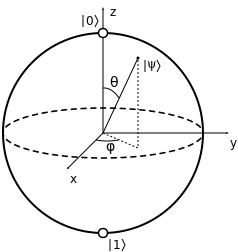
\includegraphics[scale=0.15]{Bloch_sphere.png}

  \caption{Bloch Sphere}\label{fig:bloch_sphere}
\end{figure}

Let
\[
  \hat{\eta} = \begin{pmatrix}
    \sin(\theta)\cos(\phi) \\
    \sin(\theta)\sin(\phi) \\
    \cos(\theta)
  \end{pmatrix}
\]
be a direction/point on the sphere (in spherical coordinates).  Then, the spin operator in the direction of $\hat{\eta}$ (with angles $\theta$ and $\phi$ as above) the Bloch state $\ket{\psi(\theta, \phi)}$ is an eigenfunction with positive eigenvalue $\hbar/2$.  (FIXME!  Need details!)


\section{Gates}

\begin{definition}
  A $1$-qubit \emph{gate}\index{gate} is simply an element of $\U_2(\C)$ acting on a singe qubit.  More gerenerally an $n$-qubit gate is an element of $U_{2^n}(\C)$.
\end{definition}

\begin{notation}
  \begin{enumerate}

  \item{} \emph{$X$ Gate\index{X gate@$X$ gate}}: multiplication by:
    \[
      X\index[not]{X@$X$} \idef \left(
        \begin{array}{rr}
          0 & 1 \\
          1 & 0
        \end{array}\right)
    \]
    It is basically the NOT gate, $\ket{x} \mapsto \ket{x \oplus 1}$.  So, $\alpha \ket{0} + \beta \ket{1} \mapsto \beta \ket{0} + \alpha \ket{1}$.

  \item{} \emph{$Y$ Gate\index{Y gate@$Y$ gate}}: multiplication by:
    \[
      Y\index[not]{Y@$Y$} \idef \left(
        \begin{array}{rr}
          0 & -\mi \\
          \mi & 0
        \end{array}\right)
    \]
    So, $\alpha \ket{0} + \beta \ket{1} \mapsto -\mi\beta \ket{0} + \alpha \mi\ket{1} \sim \beta \ket{0} - \alpha \ket{1}$.

  \item{} \emph{$Z$ Gate\index{Z gate@$Z$ gate}}: multiplication by:
    \[
      Z\index[not]{Z@$Z$} \idef \left(
        \begin{array}{rr}
          1 &  0\\
          0 & -1
        \end{array}\right)
    \]
    So, $\alpha \ket{0} + \beta \ket{1} \mapsto \alpha \ket{0} - \beta \ket{1}$, or $Z \ket{x} = {(-1)}^x \ket{x}$, for $x \in \F_2$.  Note then that the $Z$ gate is a \emph{phase flip}.

  \item \emph{Hadamard Gate}\index{Hadamard gate}: multiplication by
    \[
      H\index[not]{H@$H$} \idef \frac{\sqrt{2}}{2}
      \left(
        \begin{array}{rr}
          1 & 1 \\
          1 & -1
        \end{array}
      \right)
    \]
    Note that, with the Hadamard gate we have
    \begin{align*}
      \ket{0} &\mapsto \ket{+}, & \ket{+} &\mapsto \ket{0}, \\
      \ket{1} &\mapsto \ket{-}, & \ket{-} &\mapsto \ket{1}.
    \end{align*}
    So, it is a change of basis between $\{\ket{0}, \ket{1}\}$ and $\{\ket{+}, \ket{-}\}$ and back.  Moreover:
    \[
      \ket{s}\index[not]{ket s@$\ket{s}$} \idef H^{\otimes n} \ket{0}^{\otimes n} = \sum_{x \in \F_2^n} \frac{1}{2^{n/2}}\ket{x},
    \]
    and hence it changes $\ket{00 \ldots 0}$ to one of equal probabilities, i.e., an equal (unbiased) superposition of all computational basis elements.

  \item We also have the \emph{$S$ gate}\index{S gate@$S$ gate} and \emph{$T$ gate}\index{T gate@$T$ gate}:
  \[
    S\index[not]{S@$S$} \idef \left(
      \begin{array}{rr}
        1 & 0 \\
        0 & \me^{\mi \mpi /2}
      \end{array}
    \right), \qquad
    T\index[not]{T@$T$} \idef \left(
      \begin{array}{rr}
        1 & 0 \\
        0 & \me^{\mi \mpi /4}
      \end{array}
    \right)
  \]

\end{enumerate}
\end{notation}


\begin{remark}
  Note that if we have two gates $U_1$ and $U_2$, with $U_1 \sim U_2$, if they are affecting a single qubit, they can be exchanged without affecting the physical result, as they only add a global phase.  On the other hand, if they come with a \emph{controlled gate}, as seen in \cref{ssec:control_gates}, then they introduce a relative phase and \emph{cannot} be switched!
\end{remark}

\begin{remarks}
  \begin{enumerate}

  \item The $X$, $Y$, and $Z$ gates can also be denoted by $\sigma_1$, $\sigma_2$, and $\sigma_3$, respectively, and are referred to as \emph{Pauli gates}\index{Pauli gates}.

  \item Note that $Y = i XZ \sim XZ$.

  \item $XY \sim Z$, $YZ \sim X$, and $XZ \sim Y$.

  \item Note that all the matrices of these gates are their own inverses.

  \item  In fact, they are all \emph{unitary}\index{unitary}, meaning $\adj{A} = A^{-1}$ (where $\adj{A}$ is the \emph{adjoint}\index{adjoint}, i.e., the complex conjugate of the transpose of $A$).  We shall denote the set of $n \times n$ unitary complex matrices by $\un$.

  \item More over, quantum evolutions are \emph{always} unitary, and therefore preserve inner products and norms.


  \item Note that $\ket{+}$ and $\ket{-}$ have the same probabilities for $0$ and $1$ (half for each), but after applying $H$ (getting $\ket{0}$ and $\ket{1}$ respectively), they do not!

  \item Note that $S$ and $T$ introduce relative phases of $\mpi/2$ and $\mi / 4$.

  \end{enumerate}
\end{remarks}


\begin{theorem}
  If $U \in \U_2(\C)$, then
  \[
    U = \me^{\mi \chi} \left(
      \begin{array}{rr}
        \cos(\theta/2) & -\me^{\mi \lambda}\sin(\theta/2) \\
        \me^{\mi \phi} \sin(\theta/2) & \me^{\mi (\phi + \lambda)} \cos(\theta/2)
      \end{array}
    \right),
  \]
  for some $\chi, \theta, \phi, \lambda \in \R$.  (Note that $\chi$ only affects the overall phase, so it is irrelevant.)
\end{theorem}


\begin{remark}
  Most quantum algorithms start with $\ket{s}$ (equal probabilities) and then amplify the coefficient of the answer.  Then, measuring will most likely give you the correct answer.
\end{remark}


\section{Rotations}

We also have \emph{rotations}\index{rotations} around the $X$, $Y$, and $Z$ angles:
\begin{align*}
  R_X\index[not]{R sub X@$R_X$}(\theta) &\idef \exp\left( -\mi \frac{\theta}{2} X \right) =
                \left(
                \begin{array}{rr}
                  \cos(\theta/2) & -\mi\sin(\theta/2) \\
                  -\mi \sin(\theta/2) & \cos(\theta/2)
                \end{array}
                \right) \\
  R_Y\index[not]{R sub Y@$R_Y$}(\theta) &\idef \exp\left( -\mi \frac{\theta}{2} Y \right) =
                \left(
                \begin{array}{rr}
                  \cos(\theta/2) & -\sin(\theta/2) \\
                  \sin(\theta/2) & \cos(\theta/2)
                \end{array}
                \right) \\
  R_Z\index[not]{R sub Z@$R_Z$}(\theta) &\idef \exp\left( -\mi \frac{\theta}{2} Z \right) =
                \left(
                \begin{array}{cc}
                  \me^{-\mi \theta/2} & 0 \\
                  0 & \me^{\mi \theta/2}
                \end{array}
                                          \right)
                                          % \sim
                % \left(
                % \begin{array}{rr}
                %   1 & 0 \\
                %   0 & \me^{\mi \theta}
                % \end{array}
                % \right)
\end{align*}

Note that if $R$ is one of these, then:
\begin{itemize}

\item $R(0) = \idt$;

\item $R(\theta_1 + \theta_2) = R(\theta_1) R(\theta_2)$;

\item $R(2 \mpi) = - \idt \sim \idt$.

\end{itemize}


\begin{remark}
  Note that $R_Z(\pi/2) \sim S$ and $R_Z(\pi/4) \sim T$.
\end{remark}


\begin{theorem}
  If $U \in \U_2(\C)$, then
  \[
    U = \me^{\mi \chi} R_X(\theta_1) R_{Y}(\theta_2) R_X(\theta_3),
  \]
  for some $\chi, \theta_1, \theta_2, \theta_3 \in \R$.  Moreover the $X$ and $Y$ can be replaces by any two of $X$, $Y$, and $Z$.
\end{theorem}



\section{Quantum Circuits}\label{sec:circuits}

Circuits apply gates to particular qubits.  For instance:

\begin{center}
  \begin{quantikz}
    %\gategroup[wires=3,steps=10]{}
    &\lstick{$\ket{0}$} & \qw & \qw & \gate{X} & \qw
    \rstick[wires=3]{$\frac{\ket{100} + \ket{110}}{\sqrt{2}}$}
    \\
    &\lstick{$\ket{0}$} & \gate{X}& \gate{H} & \qw  & \qw
    \\
    &\lstick{$\ket{1}$} & \qw & \qw & \gate{X} & \qw
    &&&&
  \end{quantikz}
\end{center}

Breaking it down in steps:
\begin{align*}
  \ket{001}
  &\mapsto \ket{011} \\
  &\mapsto \ket{0} \otimes \left( \frac{\sqrt{2}}{2} \ket{0} - \frac{\sqrt{2}}{2} \ket{1} \right) \otimes \ket{1}
    = \frac{\sqrt{2}}{2} \ket{001} + \frac{\sqrt{2}}{2} \ket{011}\\
  &\mapsto \frac{\sqrt{2}}{2} \ket{100} + \frac{\sqrt{2}}{2} \ket{110}.
\end{align*}

So, the probability that we get $\ket{100}$ or $\ket{110}$ is $1/2$ each, and $0$ for every other state.

We can also add measurements to the circuit:
\begin{center}
  \begin{quantikz}
    %\gategroup[wires=3,steps=7]{}
    &\lstick{$\ket{0}$} & \qw & \qw & \gate{X} & \meter{} &\qw
    % \rstick[wires=3]{$\frac{|{000}\rangle + |{111}\rangle}{\sqrt{2}}$}
    \\
    &\lstick{$\ket{0}$} & \gate{X}& \gate{H} & \qw& \meter{} &\qw
    \\
    &\lstick{$\ket{1}$} & \qw & \qw & \gate{X} & \meter{} &\qw
    &&&&
  \end{quantikz}
\end{center}


\section{Multi-Qubit Gates}\label{sec:mq-gates}

\subsection{$\cnot$ Gate}

Here is the \emph{$\cnot$ Gate}\index{cnot gate@$\cnot$ Gate} (for \emph{controlled not gate}) or \emph{controlled NOT gate}\index{controlled NOT gate}: we have a control qubit and target qubit.  If the control qubit is $1$, then flip the value of the target bit.  The graphical representation is

\begin{center}
  \begin{quantikz}
    & \ctrl{1} & \qw \\
    & \targ{} &  \qw &
  \end{quantikz}
\end{center}

The dot is the control and the circle is the target.  So, if the first qubit is the control and the second is the target, then this takes:
\begin{align*}
  \ket{00} &\mapsto \ket{00}, \\
  \ket{10} &\mapsto \ket{11}, \\
  \ket{01} &\mapsto \ket{01}, \\
  \ket{11} &\mapsto \ket{10}.
\end{align*}
Or, we can represent:
\[
  \cnot \ket{x}\ket{y} \idef
  \begin{cases}
    \ket{x}\ket{y}, &\text{if $x = 0$};\\
    \ket{x}\ket{y \oplus 1}, &\text{if $x=1$}.
  \end{cases}
\]
As a matrix:
\[
  \cnot =
  \begin{pmatrix}
    1 & 0 & 0 & 0 \\
    0 & 0 & 0 & 1 \\
    0 & 0 & 1 & 0 \\
    0 & 1 & 0 & 0
  \end{pmatrix}.
\]



\begin{theorem}
  On $n$ qubits, the set
  \[
    \mathcal{G} \idef \{\text{$1$-qubit gates on any qubit}\} \cup \{\text{$\cnot$ on any two qubits}\}
  \]
  generates all gates, i.e., it generates $U_{2^n}(\C)$.
\end{theorem}


\begin{theorem}
  We have that $\dim_{\R}U_n(\C)$ is $2n^2$ (as an Euclidean space), so $\dim_{\R}\U_{n^2}(\C) = 2 \cdot {(2^n)}^2 = 2 \cdot 2^{2n} = 2 \cdot 4^n$.
\end{theorem}



\subsection{Multiple Control Gates}

We can have multiple controls for a gate.  In that case, all control qubits must be $\ket{1}$ in order for the gate to be applied to the target qubit.  For a gate $U$ on $n$ qubits, the notation for it is $C^{n-1}U$.

\textbf{Note:} These may be hard to create using only one-qubit gates and $\cnot$!  See \href{https://quantumcomputing.stackexchange.com/questions/13132/how-can-we-implement-controlled-t-gate-using-cnot-and-h-s-and-t-gates}{this Stack exchange post}.


\subsection{Toffoli Gate}

The \emph{Toffoli Gate}\index{Toffoli Gate} is $C^2X$, so it has two controls and one target.  We only switch the target, i.e., apply $X$, when \emph{both} controls are $1$.

\begin{center}
  \begin{quantikz}
    & \ctrl{2} & \qw \\
    & \ctrl{} &  \qw & \\
    & \targ{} &  \qw &
  \end{quantikz}
\end{center}

\subsection{Other Controlled Gates}\label{ssec:control_gates}

One can use the $\cnot$ gate to produce other controlled gates: $CY$, $CZ$, $CS$, $CH$.
% For example, here is the $CY$ gate:

% \begin{center}
%   \begin{quantikz}
%     & \ctrl{1} & \qw & \qw  & \qw \\
%     & \targ{} & \gate{X} & \gate{Y} &  \qw &
%   \end{quantikz}
% \end{center}

Here is a graphic representation:

\begin{center}
  \begin{quantikz}
    & \gate{S} & \qw \\
    & \ctrl{-1} &  \qw &
  \end{quantikz}
\end{center}


\section{Measuring Singular Qubits}

If we have:
\[
  \ket{\psi_0} = \frac{1}{2} \ket{00} + \frac{1}{4} \ket{01} + \frac{\sqrt{2}}{2} \ket{10} + \frac{\sqrt{3}}{4} \ket{11}
\]
and we measure the first qubit to be $1$, then the new state is
\[
  \ket{\psi_1} = c \cdot \left(  \frac{\sqrt{2}}{2} \ket{10} + \frac{\sqrt{3}}{4} \ket{11} \right),
\]
with
\[
  c^2 \left( \frac{1}{2} + \frac{3}{16} \right) = 1
\]
due to probabilities.  Hence, $c = 4/\sqrt{11}$ and
\[
  \ket{\psi_1} = \frac{4}{\sqrt{22}} \ket{10} + \frac{\sqrt{3}}{\sqrt{11}} \ket{11}.
\]


\section{Entanglement}

Consider the circuit:

\begin{center}
  \begin{quantikz}
    %\gategroup[wires=3,steps=10]{}
    &\lstick{$\ket{0}$} & \gate{H} & \ctrl{1} & \qw
    \rstick[wires=2]{$\frac{\ket{00} + \ket{11}}{\sqrt{2}}$}
    \\
    &\lstick{$\ket{0}$} & \qw & \targ{} & \qw
    &&&&
  \end{quantikz}
\end{center}

\begin{align*}
  \ket{00} &\mapsto \frac{\sqrt{2}}{2} \left(\ket{0} + \ket{1}\right) \otimes \ket{0} = \frac{\sqrt{2}}{2} \left( \ket{00} + \ket{10} \right) \\
  &\mapsto \frac{\sqrt{2}}{2} \left( \ket{00} + \ket{11} \right).
\end{align*}

Hence, if the first qubit is measured as $0$, then the second qubit must also be $0$, and similarly if it is measured as $1$, then the second must also be $1$.  So, these qubits are \emph{entangled qubits}\index{entangled qubits}.

More precisely:

\begin{definition}
  A state is \emph{entangled state}\index{entangled state} if it cannot be factored as tensor products of individual qubits.
\end{definition}

\begin{example}
  We have that
  \[
    \frac{\sqrt{3}}{2\sqrt{5}} \ket{00} + \frac{1}{2\sqrt{5}} \ket{01} + \frac{\sqrt{3}}{\sqrt{5}} \ket{10} + \frac{1}{\sqrt{5}} \ket{11} = \left(\frac{1}{\sqrt{5}}\ket{0} + \frac{2}{\sqrt{5}} \ket{1}\right) \otimes \left(\frac{\sqrt{3}}{2} \ket{0} + \frac{1}{2} \ket{1}\right)
  \]
  so that state is \emph{not} entangled.  On the other hand
  \[
    \frac{\sqrt{2}}{2}\left( \ket{000} + \ket{011} \right)
  \]
  cannot be written as a tensor product, so it is.  (Note that if we measure the second qubit, we know the state of the other two.)
\end{example}

\begin{definition}
  \begin{enumerate}

  \item Qubits are \emph{maximally entangled qubits}\index{maximally entangled qubits} if measuring one of the qubits determine the other qubits.

  \item \emph{Bell states}\index{Bell states} are some examples of maximally entangled qubits:
    \begin{itemize}[itemsep=1.3ex]

    \item $\ket{\Phi^+}\index[not]{phi plus@$\ket{\Phi^+}$} = \frac{1}{\sqrt{2}} (\ket{00} + \ket{11})$;

    \item $\ket{\Phi^-}\index[not]{phi minus@$\ket{\Phi^-}$} = \frac{1}{\sqrt{2}} (\ket{00} - \ket{11})$;

    \item $\ket{\Psi^+}\index[not]{psi plus@$\ket{\Psi^+}$} = \frac{1}{\sqrt{2}} (\ket{01} + \ket{10})$;

    \item $\ket{\Psi^-}\index[not]{psi minus@$\ket{\Psi^-}$} = \frac{1}{\sqrt{2}} (\ket{01} - \ket{10})$.

    \end{itemize}

  \item Qubits are \emph{partially entangled}\index{partially entangled} if measuring one of the qubits affect the probabilities for the other qubits.  E.g., consider
    \[
      \ket{\psi} = \frac{\sqrt{3}}{\sqrt{5}} \ket{00} + \frac{1}{\sqrt{5}} \ket{01} + \frac{1}{2\sqrt{5}} \ket{10} + \frac{\sqrt{3}}{2\sqrt{5}} \ket{11}.
    \]
    If we measure the first qubit as $0$, we get
    \[
      \ket{0} \otimes \left( \frac{\sqrt{3}}{2} \ket{0} + \frac{1}{2} \ket{1} \right),
    \]
    while if we measure the first qubit as $1$, we get
    \[
      \ket{1} \otimes \left( \frac{1}{2} \ket{0} + \frac{\sqrt{3}}{2} \ket{1} \right).
    \]

  \end{enumerate}
\end{definition}


\section{Phase Kickback}

Consider:

\begin{center}
  \begin{quantikz}
    &\lstick{$\ket{+}$} & \qw & \ctrl{1} &  \qw
    \\
    &\lstick{$\ket{v}$} & \qw & \gate{U} & \qw
    &&&&
  \end{quantikz}
\end{center}
and suppose the $\ket{v}$ is an \emph{eigenstate}\index{eigenstate} of $U$, meaning, $U \ket{v} = \me^{\mi \theta} \ket{v}$.  (Note that, due to normalization, all eigenvalues are of the form $\me^{\mi \theta}$.)

We then have
\begin{align*}
  \ket{+} \otimes \ket{v}
  &= \frac{\sqrt{2}}{2} \left( \ket{0}\otimes \ket{v} + \ket{1} \otimes \ket{v} \right) \\
  &\mapsto \frac{\sqrt{2}}{2} \left( \ket{0}\otimes \ket{v} + \ket{1} \otimes U \ket{v} \right) \\
  &= \frac{\sqrt{2}}{2} \left( \ket{0}\otimes \ket{v} + \me^{\mi \theta} \ket{1} \otimes \ket{v} \right) \\
  &= \frac{\sqrt{2}}{2} \left( \ket{0} + \me^{\mi \theta} \ket{1} \right) \otimes \ket{v}.
\end{align*}
So, $\ket{v}$ is unchanged (even though it was the target qubit), and a relative phase was applied to the control qubit.

So, if we apply a controlled gate to a target that is an eigenvector of this gate, the phase of the control qubit is changed.  This is called \emph{phase kickback}\index{phase kickback}.


\section{Superdense Coding}

Alice can send Bob two classical bits using only one qubit.  Alice and Bob start with a maximally entangled pair of qubits
\[
  \ket{\psi_0} = \frac{1}{\sqrt2}(\ket{00} + \ket{11}).
\]
Alice takes the first qubit and Bob the second.  Then, when Alice applies the first operation (depending on which two bits she wants to send Bob) and Bob the last two ($(H \otimes \idt) \circ \cnot$):
\[
  \begin{tikzcd}[cramped, sep=8ex]
    \ket{\psi_0} \arrow[r, mapsto, "\idt^{\otimes 2}"] & \frac{1}{\sqrt{2}} \left( \ket{00} + \ket{11} \right) \arrow[r, mapsto, "\cnot"] &  \frac{1}{\sqrt{2}} \left( \ket{00} + \ket{10} \right) = \ket{+} \otimes \ket{0} \arrow[r, mapsto, "H \otimes \idt"] & \ket{00} \\
    \ket{\psi_0} \arrow[r, mapsto, "X \otimes \idt"] & \frac{1}{\sqrt{2}} \left( \ket{10} + \ket{01} \right) \arrow[r, mapsto, "\cnot"] &  \frac{1}{\sqrt{2}} \left( \ket{11} + \ket{01} \right) = \ket{+} \otimes \ket{1} \arrow[r, mapsto, "H \otimes \idt"]  & \ket{01}\\
    \ket{\psi_0} \arrow[r, mapsto, "\idt \otimes Z"] & \frac{1}{\sqrt{2}} \left( \ket{00} - \ket{11} \right) \arrow[r, mapsto, "\cnot"] &  \frac{1}{\sqrt{2}} \left( \ket{00} - \ket{10} \right) = \ket{-} \otimes \ket{0} \arrow[r, mapsto, "H \otimes \idt"]  & \ket{10}\\
    \ket{\psi_0} \arrow[r, mapsto, "\idt \otimes XZ"] & \frac{1}{\sqrt{2}} \left( \ket{01} - \ket{10} \right) \arrow[r, mapsto, "\cnot"] &  \frac{1}{\sqrt{2}} \left( \ket{01} - \ket{11} \right) = \ket{-} \otimes \ket{1} \arrow[r, mapsto, "H \otimes \idt"]  & \ket{11}
  \end{tikzcd}
\]




\section{Grover's Algorithm}

Grover's algorithm is an \emph{unstructured search}, meaning, no assumption on the data that might help with searching.


\textbf{Problem statement:} given a list $[x_0, x_1, \ldots , x_{N-1}]$ that we can query (i.e., given $j$ we can read $x_j$ from the list) and some $y$, find if there is $j_0$ such that $x_{j_0} = y$ and output $j_0$ if so.

Traditionally, the search is $\mcal{O}(N)$, with expected number of queries and comparisons $(N + 1)/2$.

\textbf{Assumptions:} Assume $N = 2^n$ (or pad the list) and that $y$ is \emph{guaranteed} to be in the list.

\textbf{Recast:} We have the binary representation:
\[
  \{0, 1, 2, \ldots , 2^n - 1\} \to \F_2^n
\]
and so we can produce a function $f : \F_2^n \to \F_2$, where the domain corresponds to the binary representation of the index in the list, and the output is a boolean, such that:
\[
  f(j) =
  \begin{cases}
    1,& \text{if $x_j = y$}; \\
    0,& \text{otherwise.}
  \end{cases}
\]
So, we need to find $j$ such that $f(j) = 1$.

\textbf{Last assumption:} We have access to an \emph{oracle} (a quantum circuit) $U_f$ on $n$ qubits such that:
\[
  U_f \ket{j} = {(-1)}^{f(j)} \ket{j} =
  \begin{cases}
    - \ket{j},& \text{if $f(j)=1$}; \\
    \phantom{-}\ket{j}, & \text{otherwise}.
  \end{cases}
\]
Hence, $U_f$ allows us to check if $j$ is the index for $y$ in the list by checking for a phase change.  (\emph{Question:} Can we create such circuit in practice?)

Define
\[
  U_S \idef H^{\otimes n} \circ X^{\otimes n} \circ C^{n-1}Z \circ X^{\otimes n} \circ H^{\otimes n}.
\]
Note that, for $x \in \F_2^n$, we have
\[
  C^{n-1}Z \ket{x} =
  \begin{cases}
    - \ket{x},& \text{if $x = (1, 1, \ldots , 1)$}; \\
    \phantom{-}\ket{x}, & \text{otherwise}.
  \end{cases}
\]

Then, we have:
\begin{align*}
  U_S \ket{s}
  & =  H^{\otimes n} \circ X^{\otimes n} \circ C^{n-1}Z \circ X^{\otimes n} \circ H^{\otimes n} \circ H^{\otimes n} \ket{0}^{\otimes n} \\
  & =  H^{\otimes n} \circ X^{\otimes n} \circ C^{n-1}Z \circ X^{\otimes n} \ket{0}^{\otimes n} \\
  & =  H^{\otimes n} \circ X^{\otimes n} \circ C^{n-1}Z \circ \ket{1}^{\otimes n} \\
  & =  -H^{\otimes n} \circ X^{\otimes n} \ket{1}^{\otimes n} \\
  & =  -H^{\otimes n} \ket{0}^{\otimes n} \\
  & = - \ket{s}.
\end{align*}

\textbf{Note:} If $\ket{\psi}$ is such that $\langle \psi \mid s  \rangle = 0$, then $U_S \ket{\psi} = \ket{\psi}$.

\begin{proof}
  Since $H^{\otimes n}$ is unitary, we have that
  \[
    0 = \langle \psi \mid s  \rangle = \langle H^{\otimes n} \ket{\psi} \mid  H^{\otimes n} \ket{s} \rangle = \langle H^{\otimes n} \ket{\psi} \mid H^{\otimes s} H^{\otimes n} \ket{0}^{\otimes n} \rangle = \langle H^{\otimes n }\ket{\psi} \mid \ket{0}^{\otimes n} \rangle,
  \]
  and hence the component of $H^{\otimes n} \ket{\psi}$ in $\ket{0}^{\otimes n}$ is $0$.

  So, the component of $X^{\otimes n} \circ H^{\otimes n} \ket{\psi}$ in $\ket{1}^{\otimes n}$ is $0$, which implies that
  \[
    C^{n-1}Z \circ X^{\otimes n} \circ H^{\otimes n} \ket{\psi} =  X^{\otimes n} \circ H^{\otimes n} \ket{\psi}.
  \]
  Therefore,
  \[
    U_S \ket{\psi} = H^{\otimes n} \circ X^{\otimes n} \circ X^{\otimes n} \circ H^{\otimes n} \ket{\psi} = \ket{\psi}.
  \]
\end{proof}


\textbf{Summary}:
\begin{align*}
  \text{target state:}& \ket{j_0} & U_f \ket{j} &=
                              \begin{cases}
                                - \ket{j},& \text{if $j = j_0$;} \\
                                \phantom{-} \ket{j},& \text{otherwise (or $\langle j \mid j_0  \rangle = 0$)}.
                              \end{cases} \\
  \text{initial state:}& \ket{s} & U_S \ket{\psi} &=
                              \begin{cases}
                                - \ket{\psi},& \text{if $\ket{\psi} = \ket{s}$;} \\
                                \phantom{-} \ket{\psi},& \text{if $\langle \psi \mid s \rangle = 0$}.
                              \end{cases} \\
\end{align*}

We define \emph{Grover's oracle} as $G = - U_s U_f$.
\begin{theorem}[Grover, 1996]
  Let $k$ be a positive integer and let $\ket{\psi_k} \idef G^k \ket{s}$.  Then, when measuring, we have
  \[
    \prob(\text{getting $j_0$} \mid \psi_k) = \abs{\langle j_0 \mid \psi_k \rangle}^2 = \sin^2 \left( (2k+1) \arcsin \left( 2^{-n/2} \right) \right).
  \]
\end{theorem}



\begin{corollary}
  If we let
  \[
    k \idef \left\lfloor \frac{\mpi}{4 \arcsin(2^{-n/2})} - \frac{1}{2} \right\rceil \approx \frac{\mpi}{4} 2^{n/2} = \frac{\pi}{4} \sqrt{N},
  \]
  then
  \[
    \prob(\text{getting $j_0$} \mid \psi_k) = 1 - \mcal{O}\left( \frac{1}{N} \right).
  \]
\end{corollary}

\textbf{Takeaway:}  After about $\sqrt{N}$ queries, there is a very high probability we will get $j_0$ when measuring.

\begin{proof}[Proof of Grover's Theorem]
  Note that
  \[
    \langle j_0 \mid s \rangle = \frac{1}{2^{n/2}} \sum_{j \in \F_2^n} \langle j_0 \mid j \rangle = \frac{1}{2^{n/2}}.
  \]
  Since this inner product is small, the vectors are almost perpendicular.  Let $\phi_0$ be the angle between them.

  \begin{center}
    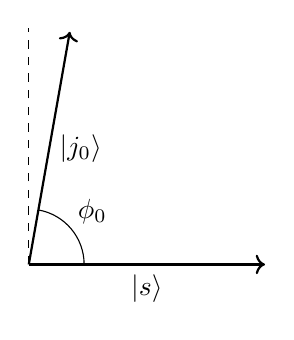
\begin{tikzpicture}
      \coordinate (O) at (0,0);
      \coordinate (P) at (3,0);
      \coordinate (Q) at (80:3);

      \draw[->, thick] (O) -- (P) node[midway,below] {$\ket{s}$};
      \draw[->, thick] (O) -- (Q) node[midway,right] {$\ket{j_0}$};
      \draw[dashed] (O) -- (0, 3);

      \draw pic["$\phi_0$",draw=black,angle radius=20,angle eccentricity=1.5]
    {angle = P--O--Q};
    \end{tikzpicture}
  \end{center}
  Then, by the inner product above, we have that $\phi_0 = \arccos(2^{-n/2})$.


  Note that $U_S$ and $U_f$ are \emph{reflections}, so $G$ is a rotation by some angle  $\alpha$.  In the plane containing $\ket{s}$ and $\ket{j_0}$, $U_f$ reflects on the line perpendicular to $\ket{j_0}$:

  \begin{center}
    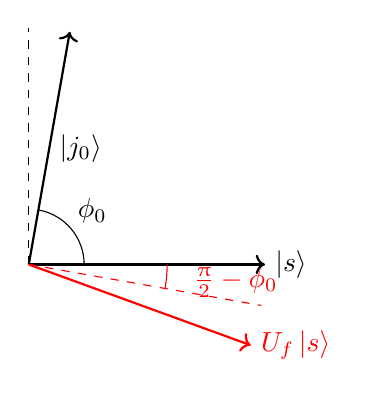
\begin{tikzpicture}
      \coordinate (O) at (0,0);
      \coordinate (P) at (3,0);
      \coordinate (Q) at (80:3);
      \coordinate (X) at (-10:3);
      \coordinate (Y) at (-20:3);

      \draw[->, thick] (O) -- (P) node[right] {$\ket{s}$};
      \draw[->, thick] (O) -- (Q) node[midway,right] {$\ket{j_0}$};
      \draw[dashed] (O) -- (0, 3);
      \draw[dashed, red] (O) -- (X);
      \draw[->, thick, red] (O) -- (Y) node[right] {$U_f \ket{s}$};

      \draw pic["$\phi_0$",draw=black,angle radius=20,angle eccentricity=1.5]
      {angle = P--O--Q};
      \draw pic["$\frac{\mpi}{2} - \phi_0$",draw,red,angle radius=50,angle eccentricity=1.5]
    {angle = X--O--P};
    \end{tikzpicture}
  \end{center}

  Similarly, $U_S$ reflects on the line perpendicular to $\ket{s}$.
  \begin{center}
    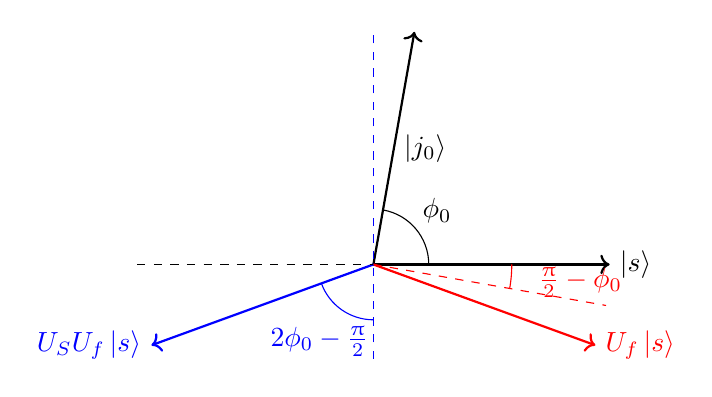
\begin{tikzpicture}
      \coordinate (O) at (0,0);
      \coordinate (P) at (3,0);
      \coordinate (R) at (0,-1.2);
      \coordinate (Q) at (80:3);
      \coordinate (X) at (-10:3);
      \coordinate (Y) at (-20:3);
      \coordinate (Z) at (200:3);

      \draw[->, thick] (O) -- (P) node[right] {$\ket{s}$};
      \draw[->, thick] (O) -- (Q) node[midway,right] {$\ket{j_0}$};
      \draw[dashed,blue] (R) -- (0, 3);
      \draw[dashed, red] (O) -- (X);
      \draw[->, thick, red] (O) -- (Y) node[right] {$U_f \ket{s}$};
      \draw[->, thick, blue] (O) -- (Z) node[left] {$U_SU_f \ket{s}$};
      \draw[dashed] (-3,0) -- (O);

      \draw pic["$\phi_0$",draw=black,angle radius=20,angle eccentricity=1.5]
      {angle = P--O--Q};
      \draw pic["$\frac{\mpi}{2} - \phi_0$",draw,red,angle radius=50,angle eccentricity=1.5]
      {angle = X--O--P};
      \draw pic["$2 \phi_0 - \frac{\mpi}{2}$",draw,blue,angle radius=20,angle eccentricity=1.7]
    {angle = Z--O--R};
    \end{tikzpicture}
  \end{center}

  Hence, we have:
  \begin{center}
    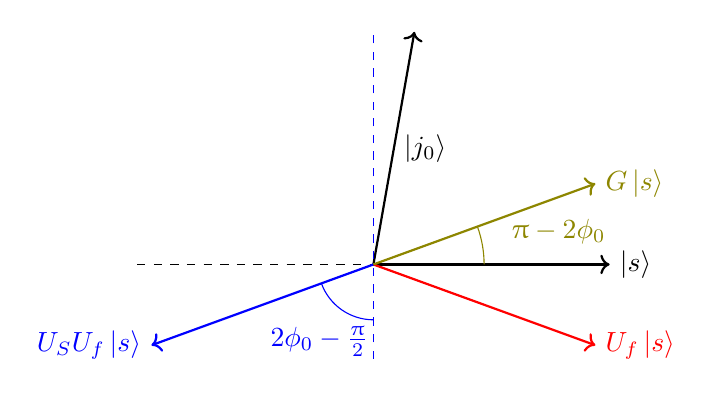
\begin{tikzpicture}
      \coordinate (O) at (0,0);
      \coordinate (P) at (3,0);
      \coordinate (R) at (0,-1.2);
      \coordinate (Q) at (80:3);
      \coordinate (X) at (-10:3);
      \coordinate (Y) at (-20:3);
      \coordinate (Z) at (200:3);
      \coordinate (W) at (200:-3);

      \draw[->, thick] (O) -- (P) node[right] {$\ket{s}$};
      \draw[->, thick] (O) -- (Q) node[midway,right] {$\ket{j_0}$};
      \draw[dashed,blue] (R) -- (0, 3);
      % \draw[dashed, red] (O) -- (X);
      \draw[dashed] (-3,0) -- (O);
      \draw[->, thick, red] (O) -- (Y) node[right] {$U_f \ket{s}$};
      \draw[->, thick, blue] (O) -- (Z) node[left] {$U_SU_f \ket{s}$};
      \draw[->, thick, olive] (O) -- (W) node[right] {$G \ket{s}$};

      % \draw pic["$\phi_0$",draw=black,angle radius=20,angle eccentricity=1.5]
      % {angle = P--O--Q};
      % \draw pic["$\frac{\mpi}{2} - \phi_0$",draw,red,angle radius=50,angle eccentricity=1.5]
      % {angle = X--O--P};
      \draw pic["$2 \phi_0 - \frac{\mpi}{2}$",draw,blue,angle radius=20,angle eccentricity=1.7]
      {angle = Z--O--R};
      \draw pic["$\mpi - 2 \phi_0$",draw,olive,angle radius=40,angle eccentricity=1.7]
      {angle = P--O--W};
    \end{tikzpicture}
  \end{center}

  Hence, $G$ is a rotation of $\alpha = \mpi - 2 \phi_0$.  Since $\phi_0$ is close to $\mpi/2$, we have that $\alpha$ is close to $0$.  So, we have:
  \begin{center}
    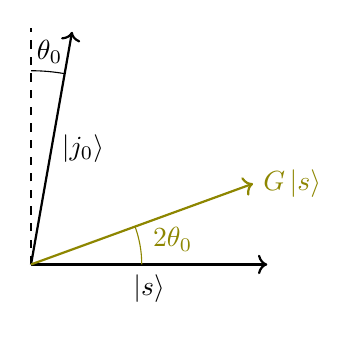
\begin{tikzpicture}
      \coordinate (O) at (0,0);
      \coordinate (P) at (3,0);
      \coordinate (R) at (0,-1.2);
      \coordinate (Q) at (80:3);
      \coordinate (X) at (-10:3);
      \coordinate (Y) at (-20:3);
      \coordinate (Z) at (200:3);
      \coordinate (W) at (200:-3);
      \coordinate (T) at (0,3);

      \draw[->, thick] (O) -- (P) node[midway,below] {$\ket{s}$};
      \draw[->, thick] (O) -- (Q) node[midway,right] {$\ket{j_0}$};
      \draw[dashed] (O) -- (0, 3);
      % \draw[dashed, red] (O) -- (X);
      % \draw[dashed] (-3,0) -- (O);
      % \draw[->, thick, red] (O) -- (Y) node[right] {$U_f \ket{s}$};
      % \draw[->, thick, blue] (O) -- (Z) node[left] {$U_SU_f \ket{s}$};
      \draw[->, thick, olive] (O) -- (W) node[right] {$G \ket{s}$};

      \draw pic["$\theta_0$",draw=black,angle radius=70,angle eccentricity=1.1]
      {angle = Q--O--T};
      % \draw pic["$\frac{\mpi}{2} - \phi_0$",draw,red,angle radius=50,angle eccentricity=1.5]
      % {angle = X--O--P};
      % \draw pic["$2 \phi_0 - \frac{\mpi}{2}$",draw,blue,angle radius=20,angle eccentricity=1.7]
      % {angle = Z--O--R};
      \draw pic["$2 \theta_0$",draw,olive,angle radius=40,angle eccentricity=1.3]
      {angle = P--O--W};
    \end{tikzpicture}
  \end{center}

  Therefore, the angle for $\ket{\psi_k} \idef G^k \ket{s}$ is $2k \theta_0$.  Hence, the angle between $\ket{\psi_k}$ and $\ket{j_0}$ is $\phi_0 - 2k \theta_0 = (2k+1) \phi_0 - k \mpi$.  Noting that
  \begin{itemize}

  \item $\phi_0 = \arccos(2^{-n/2})$,

  \item $\cos(x + \mpi/2) = -\sin(x)$, and

  \item $\mpi/2 - \arccos(\mpi/x) = \arcsin(x)$,

  \end{itemize}
  we have
  \begin{align*}
    \abs{\langle j_0 \mid \psi_k \rangle}^2
    &= \cos^2((2k+1)\phi_0 - k\mpi) \\
    &=\cos^2(-(2k+1)(\mpi/2 - \phi_0) + \mpi/2) \\
    &= \sin^2((2k+1) \arcsin(2^{-n/2})).
  \end{align*}


\end{proof}


\section{Quantum Fourier Transform}


(More of a quantum ``subroutine''.)


\begin{lemma}\label{lemma:expsum}
  Let $\zeta_N \idef \me^{2 \mpi \mi/N}$, with $N \geq 2$, and $a \in \R$.  Then we have
  \[
    \sum_{b=0}^{N-1} \zeta_N^{ab} =
    \begin{cases}
      N, & \text{if $a \in \Z$ and $a \equiv 0 \pmod{N}$}; \\
      0, & \text{if $a \in \Z$ and $a \not\equiv 0 \pmod{N}$}; \\
      \frac{{\left(\zeta_N^{a}\right)}^N - 1}{\zeta_N - 1}, & \text{if $a \not\in \Z$}.
    \end{cases}
  \]
\end{lemma}

\begin{proof}
  We have that $\zeta_N^a = 1$ if and only if $a \in \Z$ and $a \equiv 0 \pmod{N}$, in which case the result is trivial.  So, suppose that $\zeta_N^a \neq 1$.  Then:
  \[
    \sum_{b=0}^{N-1} {\left(\zeta_N^a\right)}^b = \frac{\zeta_N^{aN} - 1}{\zeta_N^a - 1}.
  \]
  If $a \in \Z$, then ${\left( \zeta_N^a \right)}^N = {\left( \zeta_N^N \right)}^a = 1$.
\end{proof}


\subsection{Discrete Fourier Transform}

\begin{definition}
  Let $f : \Z/{N}\Z \to \C$ and $\zeta \idef \me^{2\mpi\mi/N}$.  Then the \emph{Discrete Fourier Transform (DFT)}\index{Discrete Fourier Transform (DFT)} is defined as
  \[
    \ft(f)(z) \idef \frac{1}{\sqrt{N}} \sum_{x=0}^{N-1} \zeta_N^{xz} f(x).
  \]
\end{definition}

It decomposes $f$ into periodic functions.


\begin{proposition}
  We have:
  \begin{enumerate}

  \item $\ft$ is linear.

  \item \emph{Parseval identity}\index{Parseval identity}: if
    \[
      \langle f_1 \mid f_2 \rangle \idef \sum_{x=0}^{N-1} \bar{f}_1(x) f_2(x),
    \]
    then
    \[
      \langle \ft(f_1) \mid \ft(f_2) \rangle = \langle f_1 \mid f_2 \rangle,
    \]
    i.e., $\ft$ is unitary.

  \item Let $k \in \Z/{N}\Z$ and define the translation
    \[
      T_k(f)(x) \idef f(x - k).
    \]
    Then,
    \[
      T_k(\ft(f))(z) = \zeta_N^{kz} \ft(T_k(f))(z).
    \]

  \end{enumerate}
\end{proposition}

\begin{proof}
  Let $\zeta_k \idef \me^{2 \mpi \mi/k}$.   For Parseval's identity, using~\vref{lemma:expsum} we have:
  \begin{align*}
    \langle \ft(f_1) \mid \ft(f_2) \rangle
    &= \sum_{x=0}^{N-1} \left[ \frac{1}{\sqrt{N}} \sum_{x_1=0}^{N-1} \zeta_N^{-x_1x} \bar{f}_1(x_1)\right] \cdot \left[ \frac{1}{\sqrt{N}} \sum_{x_2=0}^{N-1} \zeta_N^{x_2x} \bar{f}_2(x_2)\right] \\
    &= \frac{1}{N} \sum_{x=0}^{N-1} \sum_{x_1, x_2=0}^{N-1} \zeta_N^{x(x_2 - x_1)} \bar{f}_1(x_1) f_2(x_2) \\
    &= \frac{1}{N} \sum_{x=0}^{N-1} \sum_{x_1=0}^{N-1} \bar{f}_1(x_1) f_2(x_1) \\
    &= \frac{1}{N} N \sum_{x_1=0}^{N-1} \bar{f}_1(x_1) f_2(x_1) \\
    &= \langle f_1 \mid f_2 \rangle.
  \end{align*}
\end{proof}


\subsection{Quantum Fourier Transform}

\begin{definition}
  Let $N \idef 2^n$, $\zeta_N \idef \me^{2 \mpi \mi/ N}$ and
  \[
    \ket{\psi} = \sum_{x=0}^{N-1} \psi(x) \ket{x}_n, \quad \psi : \Z/{N}\Z \to \C, \; \left\| \psi \right\| = 1.
  \]
  Then,
  \begin{align*}
    \qft \ket{\psi}
    &\idef \sum_{z=0}^{2^n-1}\ft(\psi)(z) \ket{z}_n \\
    &= \frac{1}{2^{n/2}}  \sum_{z=0}^{2^n - 1}\left[ \sum_{x=0}^{2^n-1} \zeta_{2^n}^{xz} \psi(x)\right] \ket{z}_n \\
    &= \frac{1}{2^{n/2}}  \sum_{x=0}^{2^n - 1} \psi(x) \left[ \sum_{z=0}^{2^n-1} \zeta_{2^n}^{xz} \ket{z}_n \right].
  \end{align*}
\end{definition}


In particular,
\[
  \qft \ket{x}_n = \frac{1}{2^{n/2}} \sum_{z=0}^{2^n-1} \zeta_{2^n}^{xz} \ket{z}_n
\]

Also note that
\[
  \qft^{-1} \ket{x}_n = \adj{\qft} \ket{x}_n = \frac{1}{2^{n/2}} \sum_{z=0}^{2^n-1} \zeta_{2^n}^{-xz} \ket{z}_n
\]

Indeed, using Lemma~\ref{lemma:expsum} again:
\begin{align*}
  \qft^{-1} \qft \ket{x}_n
  &=  \frac{1}{2^{n/2}} \sum_{z=0}^{2^n-1} \zeta_{2^n}^{xz} \left[  \frac{1}{2^{n/2}} \sum_{y=0}^{2^n-1} \zeta_{2^n}^{-yz} \ket{y}_n \right] \\
  &= \frac{1}{2^n} \sum_{y=0}^{2^n-1} \left[ \sum_{z=0}^{2^n - 1} \zeta_{2^n}^{z(x-y)}\right] \ket{y}_n \\
  &= \ket{x}_n.
\end{align*}

\begin{remark}
  One can compute $\ft(f)$ from $f$ using the \href{https://en.wikipedia.org/wiki/Fast_Fourier_transform}{fast Fourier transform} in $\mcal{O}(\log_2(N) N)$ time.
\end{remark}

\textbf{Fact:} There are quantum circuits for the quantum Fourier transform using $\mcal{O}(n^2) = \mcal{O}({(\log_2(N))}^2)$ gates, using only $1$-qubit gates and $\cnot$ gates.  (See Nielsen-Chuang pg.~217 for a ``good'' exact implementation.)


\begin{definition}
  \emph{Ancillas}\index{Ancillas} (or ancilla qubits) are extra qubits used in the quantum circuit.
\end{definition}


\subsection{Application: Adder Circuit}

We will need the following definition:

\begin{definition}
  Let $\zeta_{2^n} \idef \me^{2 \mpi \mi/2^n}$.  We define the \emph{$P$ gate}\index{P gate@$P$ gate}:
  \[
    P(k) \ket{x}_n \idef \zeta_{2^n}^{xk} \ket{x}_n.
  \]
\end{definition}


\begin{definition}
  For $k \in \Z/{2^n}\Z$, define the \emph{plus $k$ adder}\index{plus $k$ adder}
  \[
    A_k \ket{x}_n \idef \ket{x + k}_n.
  \]
\end{definition}


\begin{align*}
  A_k \adj{\qft} \ket{x}_n
  &= \frac{1}{2^{n/2}} \sum_{z=0}^{2^n - 1} \zeta_{2^n}^{-xz} \ket{z + k}_n \\
  &= \frac{1}{2^{n/2}} \sum_{z=0}^{2^n - 1} \zeta_{2^n}^{-x(z-k)} \ket{z}_n \\
  &= \frac{1}{2^{n/2}} \zeta_{2^n}^{xk }\sum_{z=0}^{2^n - 1} \zeta_{2^n}^{-xz} \ket{z}_n \\
  &= \zeta_{2^n}^{xk} \adj{\qft} \ket{x}_n,
\end{align*}
i.e.,
\begin{equation}
  \label{eq:qftak}
  (\qft \circ A_k \circ \adj{\qft}) \ket{x}_n = \zeta_{2^n}^{xk} \ket{x}_n = P(k) \ket{x}_n,
\end{equation}
or
\begin{equation}\label{eq:ak}
  A_k = \adj{\qft} \circ P(k) \qft.
\end{equation}
(So, \emph{shift} is turned in to \emph{phase})



The $P$ gate is easy to implement: remembering that
\[
  R_Z(\theta) =
  \left(
    \begin{array}{cc}
      \me^{-\mi \theta/2} & 0 \\
      0 & \me^{\mi \theta/2}
    \end{array}
  \right) = \me^{-\mi \theta/2}
  \begin{pmatrix*}[c]
    1 & 0 \\
    0 & \me^{\mi \theta}
  \end{pmatrix*},
\]
the circuit
\begin{center}
  \begin{quantikz}
    & \lstick{$\ket{x_0}$} & \qw & \gate[5, nwires=4]{P(k)} & \qw \\
    & \lstick{$\ket{x_1}$} & \qw  & & \qw \\
    & \lstick{$\ket{x_2}$} &\qw & & \qw\\
    & \lstick{$\ \vdots \ $} & & & \qw \\
    & \lstick{$\ket{x_{n-1}}$} & \qw & & \qw
  \end{quantikz}
\end{center}
up to a global phase factor, is the same as the $n$ one-qubit gates
\begin{center}
  \begin{quantikz}
    & \lstick{$\ket{x_0}$} & \qw & \gate{R_Z(\mpi k/2^{n-1})} & \qw \\
    & \lstick{$\ket{x_1}$} & \qw  &\gate{R_Z(\mpi k /2^{n-2})} & \qw \\
    & \lstick{$\ket{x_2}$} &\qw & \gate{R_Z(\mpi k /2^{n-3})}& \qw\\
    & \lstick{$\ \vdots \ $} & & & & \\
    & \lstick{$\ket{x_{n-1}}$} & \qw & \gate{R_Z(\mpi k)}& \qw
  \end{quantikz}
\end{center}
So, using~\cref{eq:ak}, and assuming that $\qft$ can be implemented, we can also implement $A_k$.

\begin{proof}
  Let
  \[
    x = x_0 + x_1 \cdot 2 + x_2 \cdot 2^2 + \cdots + x_{n-1} \cdot 2^{n-1} = \sum_{r=0}^{n-1} x_r 2^r.
  \]
  Then,
  \begin{equation}\label{eq:exp1}
    \exp\left(\frac{2 \mpi \mi}{2^n} xk \right) = \exp\left(k \mpi \mi \sum_{r=0}^{n-1} \frac{1}{2^{n-r-1}} x_r\right)
  \end{equation}

  Also, note that for a qubit $x_r$, we have
  \[
    R_Z(\theta) \ket{x_r} = \me^{-\mi \theta/2} \me^{\mi \theta x_r} \ket{x_r}.
  \]
  So,
  \[
    R_Z\left(\frac{k \mpi}{2^{n-1-r}}\right) \ket{x_r} = \exp\left(-\frac{k \mpi \mi}{2^{n-r}}\right) \cdot \exp\left(\frac{k \mpi \mi}{2^{n-1-r}} x_r\right) \ket{x_r}.
  \]

  Therefore:
  \begin{align*}
    \bigotimes_{r=0}^{n-1}R_Z\left(\frac{k \mpi} {2^{n-1-r}}\right) \ket{x_r}
    &= \bigotimes_{r=0}^{n-1} \exp\left(-\frac{k \mpi \mi}{2^{n-r}}\right) \cdot \exp\left(\frac{k \mpi \mi}{2^{n-1-r}} x_r\right) \ket{x_r} \\
    &= \left[\prod_{r=0}^{n-1} \exp\left(-\frac{k \mpi \mi}{2^{n-r}}\right) \cdot \prod_{r=0}^{n-1}  \exp\left(\frac{k \mpi \mi}{2^{n-1-r}} x_r\right)\right] \ket{x}_n \\
    &= \left[\exp\left(-\frac{k \mpi \mi}{2^n} \sum_{r=0}^{n-1} 2^r\right) \cdot \exp\left(k \mpi \mi \sum_{r=0}^{n-1}\frac{1}{2^{n-1-r}} x_r\right)\right] \ket{x}_n \\
    &= \exp\left(-\frac{(2^n-1) k \mpi \mi}{2^n}\right) \cdot \exp\left(\frac{2 \mpi \mi}{2^n} xk \right) \ket{x}_n \\
    &= \exp\left(-\frac{(2^n-1) k \mpi \mi}{2^n}\right) \cdot P(k) \ket{x}_n.
  \end{align*}
  So, indeed the last circuit gives, up to a global phase, the $P(k)$ gate.
\end{proof}


\section{Quantum Phase Estimation}

\subsection{Fejér States}

What happens if we replace $k \in \Z$ in $A(k)$ by some $k \in  \R$?

\begin{definition}
  For $n$ bits and $k \in \R$, define $\ket{k}_F\index[not]{ket k of F@$\ket{k}_F$}$, the \emph{$k$-th Fejér state}\index{Fejér state} as
  \begin{align*}
    \ket{k}_F
    &\idef \adj{\qft} \circ P(k) \circ \qft \ket{0}_n \\
    &= \sum_{z=0}^{2^n-1} \exp\left(\mpi \mi (1 - 1/2)(k - z)\right) \frac{\sin(\mpi(k-z))}{2^n \sin(\mpi (k-z)/ 2^n)} \ket{z}_n.
  \end{align*}
\end{definition}

Then, for $x \in \{0, 1, \ldots, 2^n-1\}$, we have
\[
  \prob(x \mid \ket{k}_F) = \abs{\langle x \mid k  \rangle_F}^2 = \frac{\sin^2(\mpi(k -x))}{4^n \sin^2(\mpi(k-x)/2^n)},
\]
the \emph{Fejér kernel}\index{Fejér kernel}.

\Vref{fig:fejer_kernel} shows the graph of the Fejér kernel
\[
   \frac{\sin^2(\mpi(k -x))}{4^n \sin^2(\mpi(k-x)/2^n)}
\]
for $n = 5$ and $k = 17.3$.

\begin{figure}
  \centering
  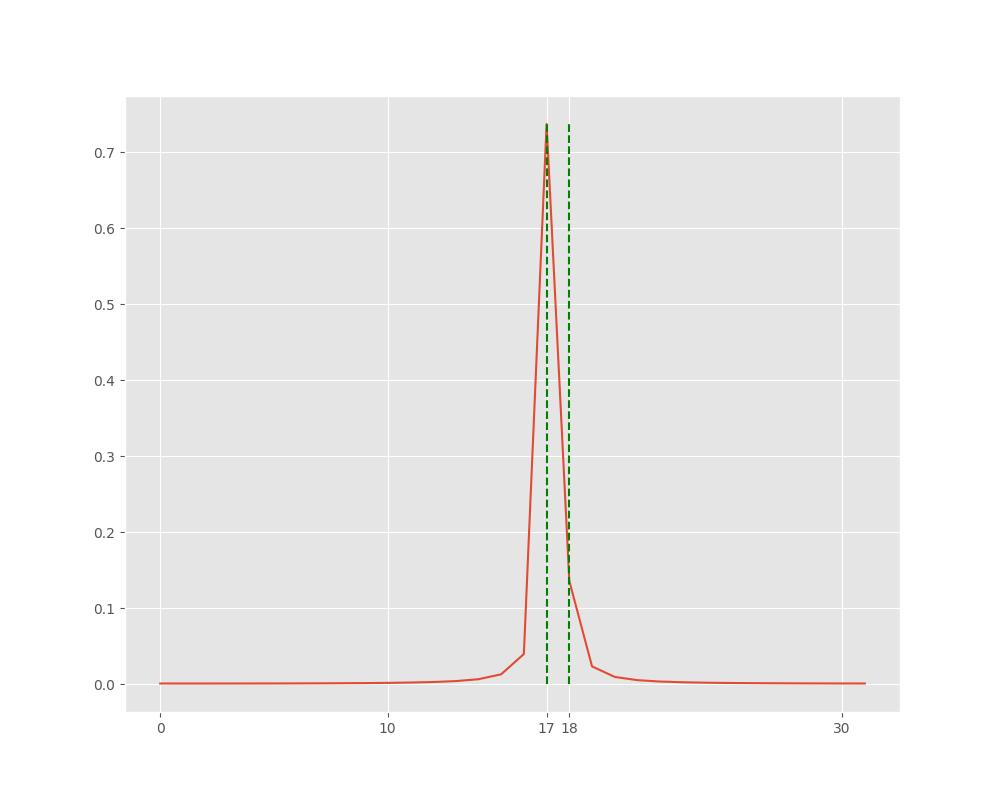
\includegraphics[scale=0.6]{fejer_kernel.jpg}
  \caption{Ferjér kernel for $k=17.3$ and $n=5$.}
  \label{fig:fejer_kernel}
\end{figure}


If we let $k = x_0 + r$, where $x_0 = \lfloor k \rceil$, so $r \in [-1/2, 1/2]$, then
\[
  \prob(x_0 \mid \ket{k}_F) = \frac{\sin^2(\mpi r)}{4^n \sin^2(\mpi r/2^n)} \geq \frac{4}{\mpi^2} \approx 0.41,
\]
and in fact
\[
   \prob(\lfloor x \rfloor \mid \ket{k}_F) +  \prob(\lceil x \rceil \mid \ket{k}_F) \geq \frac{8}{\mpi^2} \approx 0.82.
\]


\subsection{Quantum Phase Estimator/Digitizer}

Let $\mcal{H}$ be the Hilbert space of $n$-qubit states.  Given
\begin{itemize}

\item an implementation of an unitary operator $U$;

\item an \emph{eigenstate} $\ket{\psi} \in \mcal{H}$ of $U$, with $U \ket{\psi} = \me^{2 \pi \mi \theta} \ket{\psi}$, with $0 \leq \theta < 1$;

\end{itemize}
we want to find or estimate $\theta$.

\begin{remark}
  Note that $\ket{\psi} \sim \me^{2 \pi \mi \theta} \ket{\psi}$, so physically there is no difference (and hence asking for $\theta$, as is, is not a proper question). On the other hand, when we have a controlled gate $CU$ given by
  \[
    CU( \ket{a} \ket{\psi}) = \ket{a} U^a \ket{\psi} \quad \text{(for $a \in \F_2$)},
  \]
  i.e.,
  \[
    CU( \alpha \ket{0} \ket{\psi} + \beta \ket{1} \ket{\psi}) = \alpha \ket{0} \ket{\psi} + \beta \me^{2 \pi \mi \theta} \ket{1} \ket{\psi},
  \]
  then $\theta$ is relevant.
\end{remark}

\begin{definition}
  We define the $n$-qubit \emph{quantum phase estimator}\index{quantum phase estimator} for $\ket{\psi}$ as:
  \begin{center}
    \begin{quantikz}
      & \lstick{$\ket{0}$} & \qw & \gate[5, nwires=4]{H} & \ctrl{5} \qw & \qw & \qw & \qw & \qw & \cdots & \qw & \gate[5, nwires=4]{\qft} & \meter{} & \qw \\
      & \lstick{$\ket{0}$} & \qw  & \qw & \qw & \qw & \ctrl{4} & \qw & \qw & \cdots & \qw & \qw & \meter{} & \qw \\
      & \lstick{$\ket{0}$} &\qw & \qw & \qw & \qw & \qw & \ctrl{3} & \qw & \cdots & \qw & \qw & \meter{} & \qw \\
      & \lstick{$\ \vdots \ $} & & & \qw & \qw & \qw & \qw & \qw & \cdots & \qw & \meter{} & \qw \\
      & \lstick{$\ket{0}$} & \qw & \qw & \qw & \qw & \qw & \qw & \qw & \cdots & \ctrl{1} & \qw & \meter{} & \qw \\
      & \lstick{$\ket{\psi}$} & \qw & \qw & \gate{U} & \qw & \gate{U^2} & \gate{U^{2^2}} & \qw & \cdots & \gate{U^{2^{n-1}}} & \qw & \qw & \qw
    \end{quantikz}
  \end{center}
\end{definition}

We then have that
\[
  \qpe \ket{0}_n \ket{\psi} = \ket{2^n \theta}_F \ket{\psi}.
\]
Hence, measuring the first $n$ qubits, we get either $\lfloor 2^n \theta \rfloor$ or $\lceil 2^n \theta \rceil$ with probability at least $82\%$.  Pick the most likely $x_{\theta} \in \Z$ and then $\theta \approx x_{\theta} / 2^n$.

\printindex[not]
\printindex
\end{document}

% %%%%%%%%%%%%%%%%%%%%%%%%%%%%%%%%%%%%%%%%%%%%%%%%%%%%%%%%%%%
